\section{Digitala kretsar}
\index{digitala kretsar}
\label{digitala kretsar}

Digital elektronik förekommer i all modern utrustning för radio- och
telekommunikation. Ämnet är mycket omfattande och här redogörs endast
för några grundläggande digitala funktioner.

I \emph{analogtekniken} kan under ett förlopp förekomma oändligt många
nivåer, till exempel spänningar mellan noll och ett högsta värde.

I digitaltekniken förekommer bara ett bestämt antal tillstånd. I det
enklaste digitala systemet finns två tillstånd, till exempel 0 och 1
eller Till och Från eller Hög och Låg eller Fel och Rätt.

Ett system med endast två tillstånd kallas binärt. En lampa som tänds
eller släcks med en enkel strömställare är ett binärt system.
Strömställaren kan ha olika utföranden. Den kan vara en mekanisk
kontakt som är styrd för hand eller av en reläspole. Den kan också
vara en transistor eller annan anordning.

\subsection{Transistorn som strömställare}

\begin{figure}
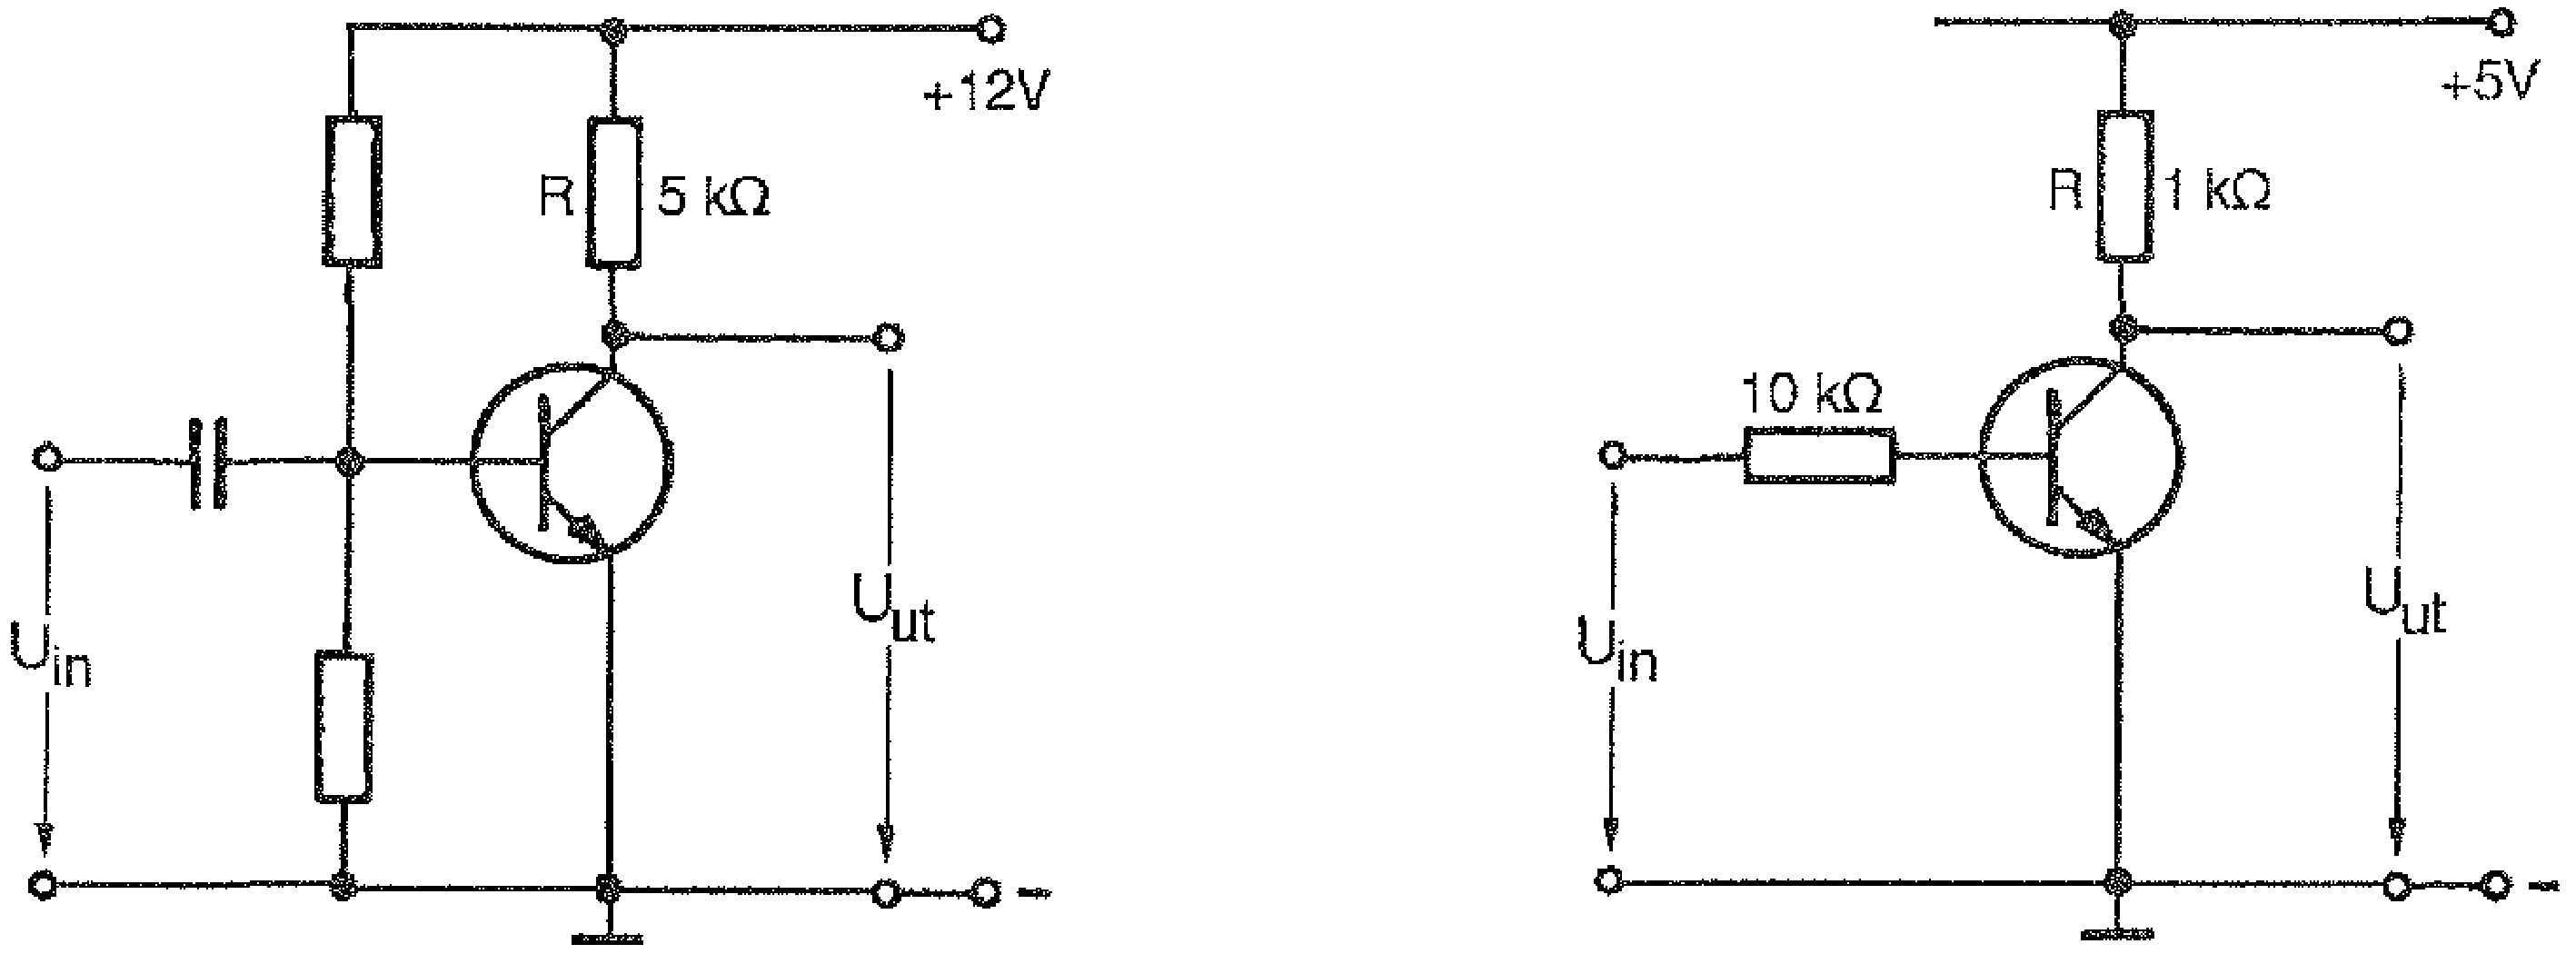
\includegraphics[width=\textwidth]{images/cropped_pdfs/bild_2_2-35.pdf}
\caption{Transistorn som analog förstärkare respektive digital strömställare}
\label{fig:BildII2-35}
\end{figure}

Bild \ref{fig:BildII2-35} visar två transistorkopplingar. Den till
vänster är en analog förstärkare för växelspänning. Om det på grund av
en viss basspänning flyter en kollektorström av 1~mA och
kollektorresistorn har värdet 5\,k\(\Omega\), blir spänningsfallet
över denna resistor 5~V. Eftersom matningsspänningen är 12\,V, blir
spänningen 7\,V mellan kollektorn och minuspolen.

Kopplingen till höger fungerar som en binär strömställare. Antag att
insignalen intar ett av två spänningstillstånd, antingen 0\,V (låg)
eller 5\,V (hög). När inspänningen är till exempel 5\,V, flyter så
mycket basström genom basresistorns 10\,k\(\Omega\) att transistorn
blir fullt utstyrd.

Därmed är spänningen mellan kollektor och emitter, det vill säga
utspänningen, nära 0\,V (0,1 till 0,2\,V beroende på transistortyp).
Man säger då att utgången är låg (L) eller 0 (noll).

Om däremot inspänningen är 0\,V, spärras kollektorströmmen och
utspänningen blir nära 5\,V. Man säger då att utgången är hög (H)
eller 1.

För NPN-transistorn i bilden gäller att hög inspänning ger låg
utspänning och vice versa.

Denna logiska funktion kallas inverterande.

\subsubsection{NOT-gate eller inverterande grind}
\index{inverterande grind}
\index{NOT-gate}

\begin{marginfigure}
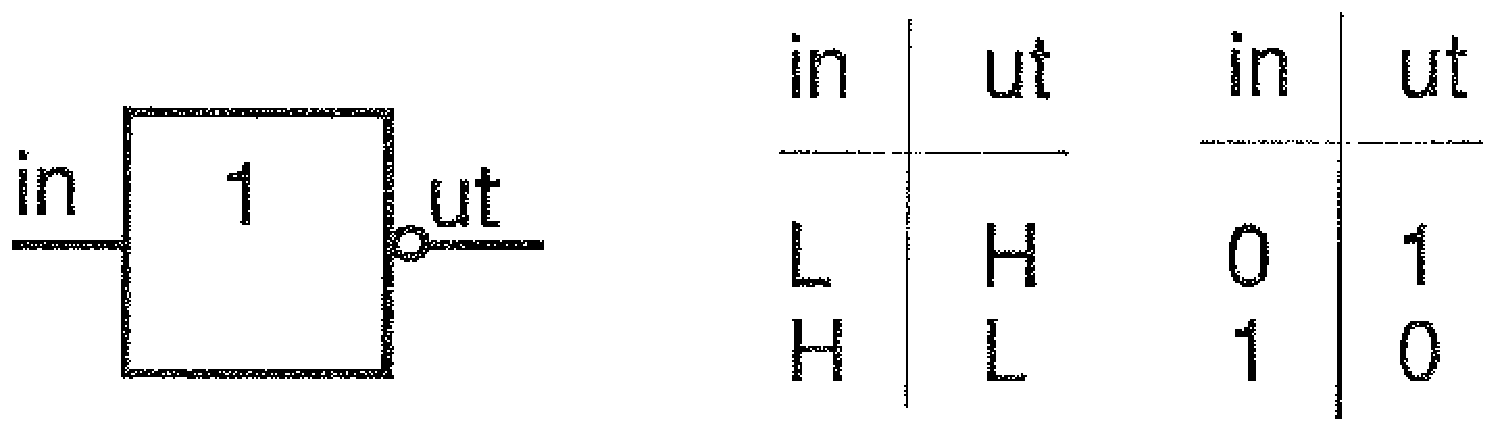
\includegraphics[width=\textwidth]{images/cropped_pdfs/bild_2_2-36.pdf}
\caption{NOT-gate}
\label{fig:BildII2-36}
\end{marginfigure}

Logiska funktioner beskrivs med internationella symboler. En ring vid
utgången betyder att utspänningens nivå är motsatt inspänningens
vilket illustreras i bild \ref{fig:BildII2-36}. Sambandet mellan in-
och utnivåerna beskrivs med en \emph{sanningstabell}.

\subsection{Villkorskretsar -- s.k. grindar}

Det finns olika sätt att bygga grindar. Idag är de flesta grindarna
elektroniska lösningar. Därutöver finns elektromekaniska grindar i
form av strömbrytare och reläkontakter.

Föregångarna till de elektroniska televäxlarna (AXE med flera) var
stora system av mestadels elektromekaniska reläer.

Att överskådligt förklara arbetssättet i de vanligaste grindarna görs
enklast med reläsymboler. En reläkontakt kan då motsvara en transistor
eller en diod. Reläspolar kan motsvara logiska nivåer i insignaler.

Elektriska kontakter kan vara normalt öppna och sluter vid påverkan
(slutande kontakt). Alternativt kan de vara normalt slutna och öppnar
vid påverkan (brytande kontakt). I kretsscheman visas kontaktlägena
vid systemet i vila.

Av bild \ref{fig:BildII2-37} framgår att samma villkor kan skapas med
slutande alternativt brytande kontakter. Observera placeringen av
resistorn på kretsens utgångssida i respektive fall. När resistorn
ligger närmast pluspolen kallas den pull-up. När den ligger närmast
minuspolen kallas den pull-down. I båda fallen definierar resistorn
den logiska nivån.

\subsubsection{OCH-grind eller AND-gate}
\index{AND-gate}

\begin{figure}
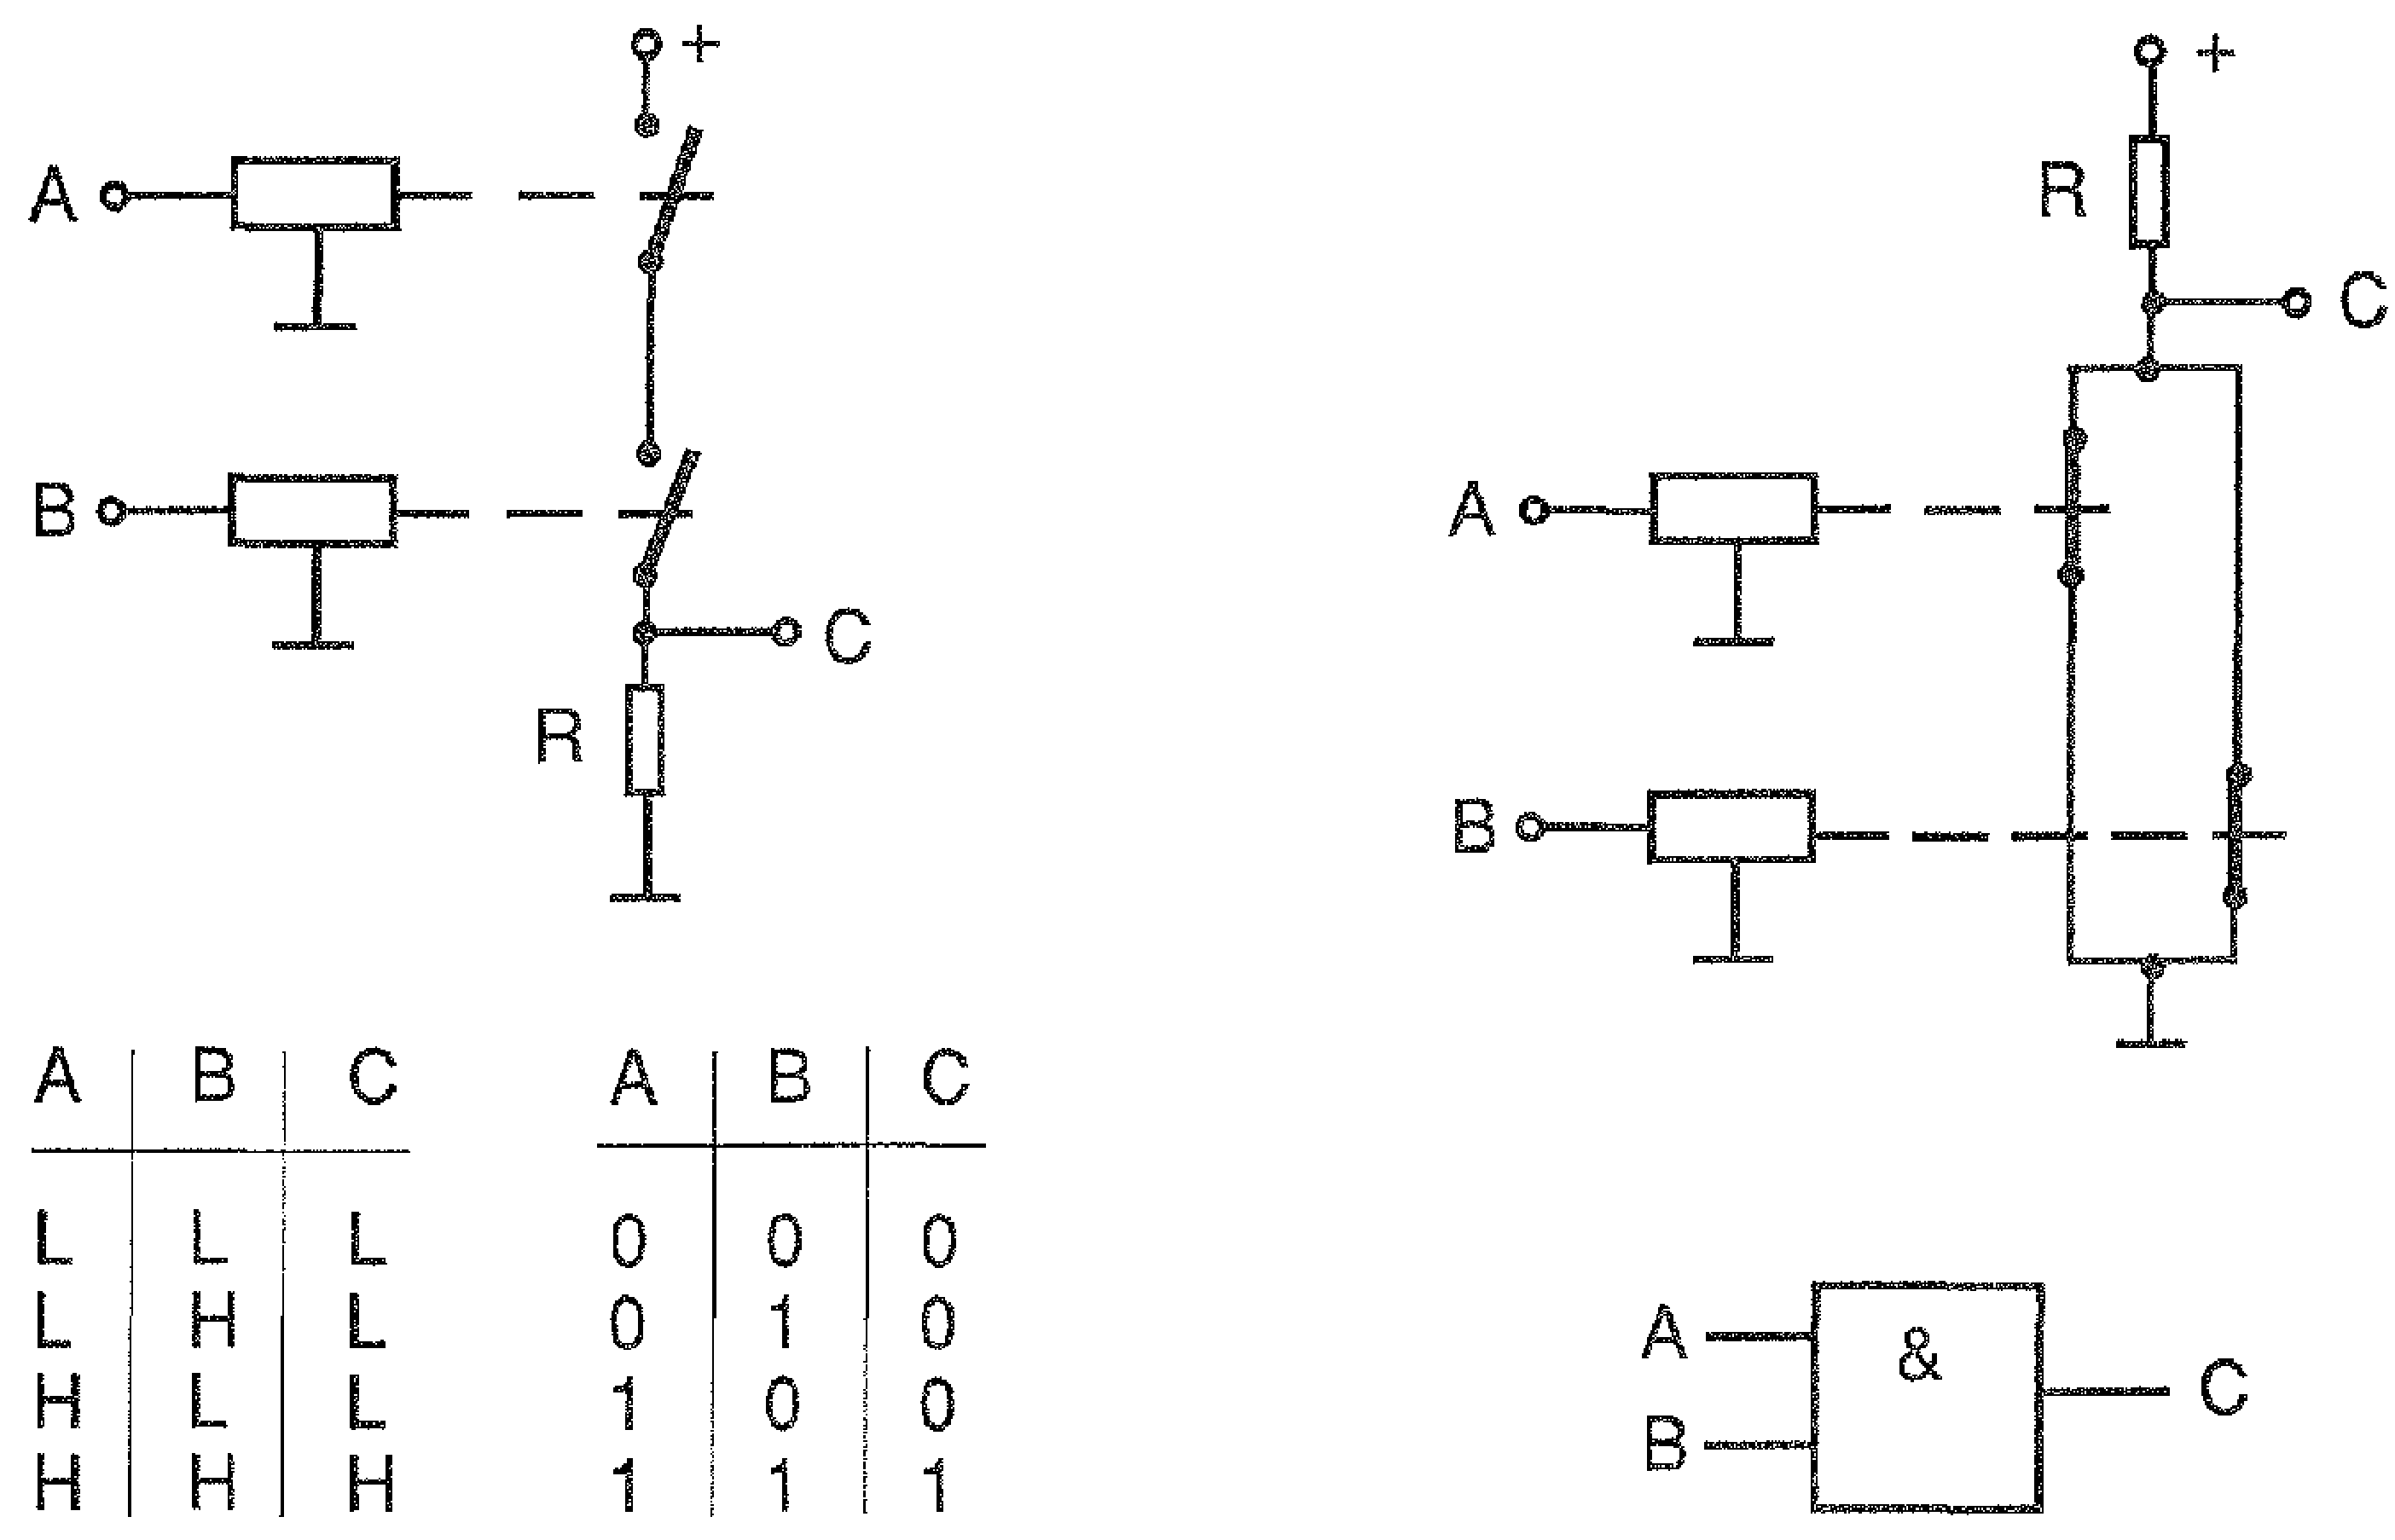
\includegraphics[width=\textwidth]{images/cropped_pdfs/bild_2_2-37.pdf}
\caption{OCH-grind (AND-gate)}
\label{fig:BildII2-37}
\end{figure}

Sanningstabellen i bild \ref{fig:BildII2-37} säger att när alla insignaler
är 1 så är utsignalen också 1.

\subsubsection{ELLER-grind eller OR-gate}
\index{OR-gate}

\begin{figure}
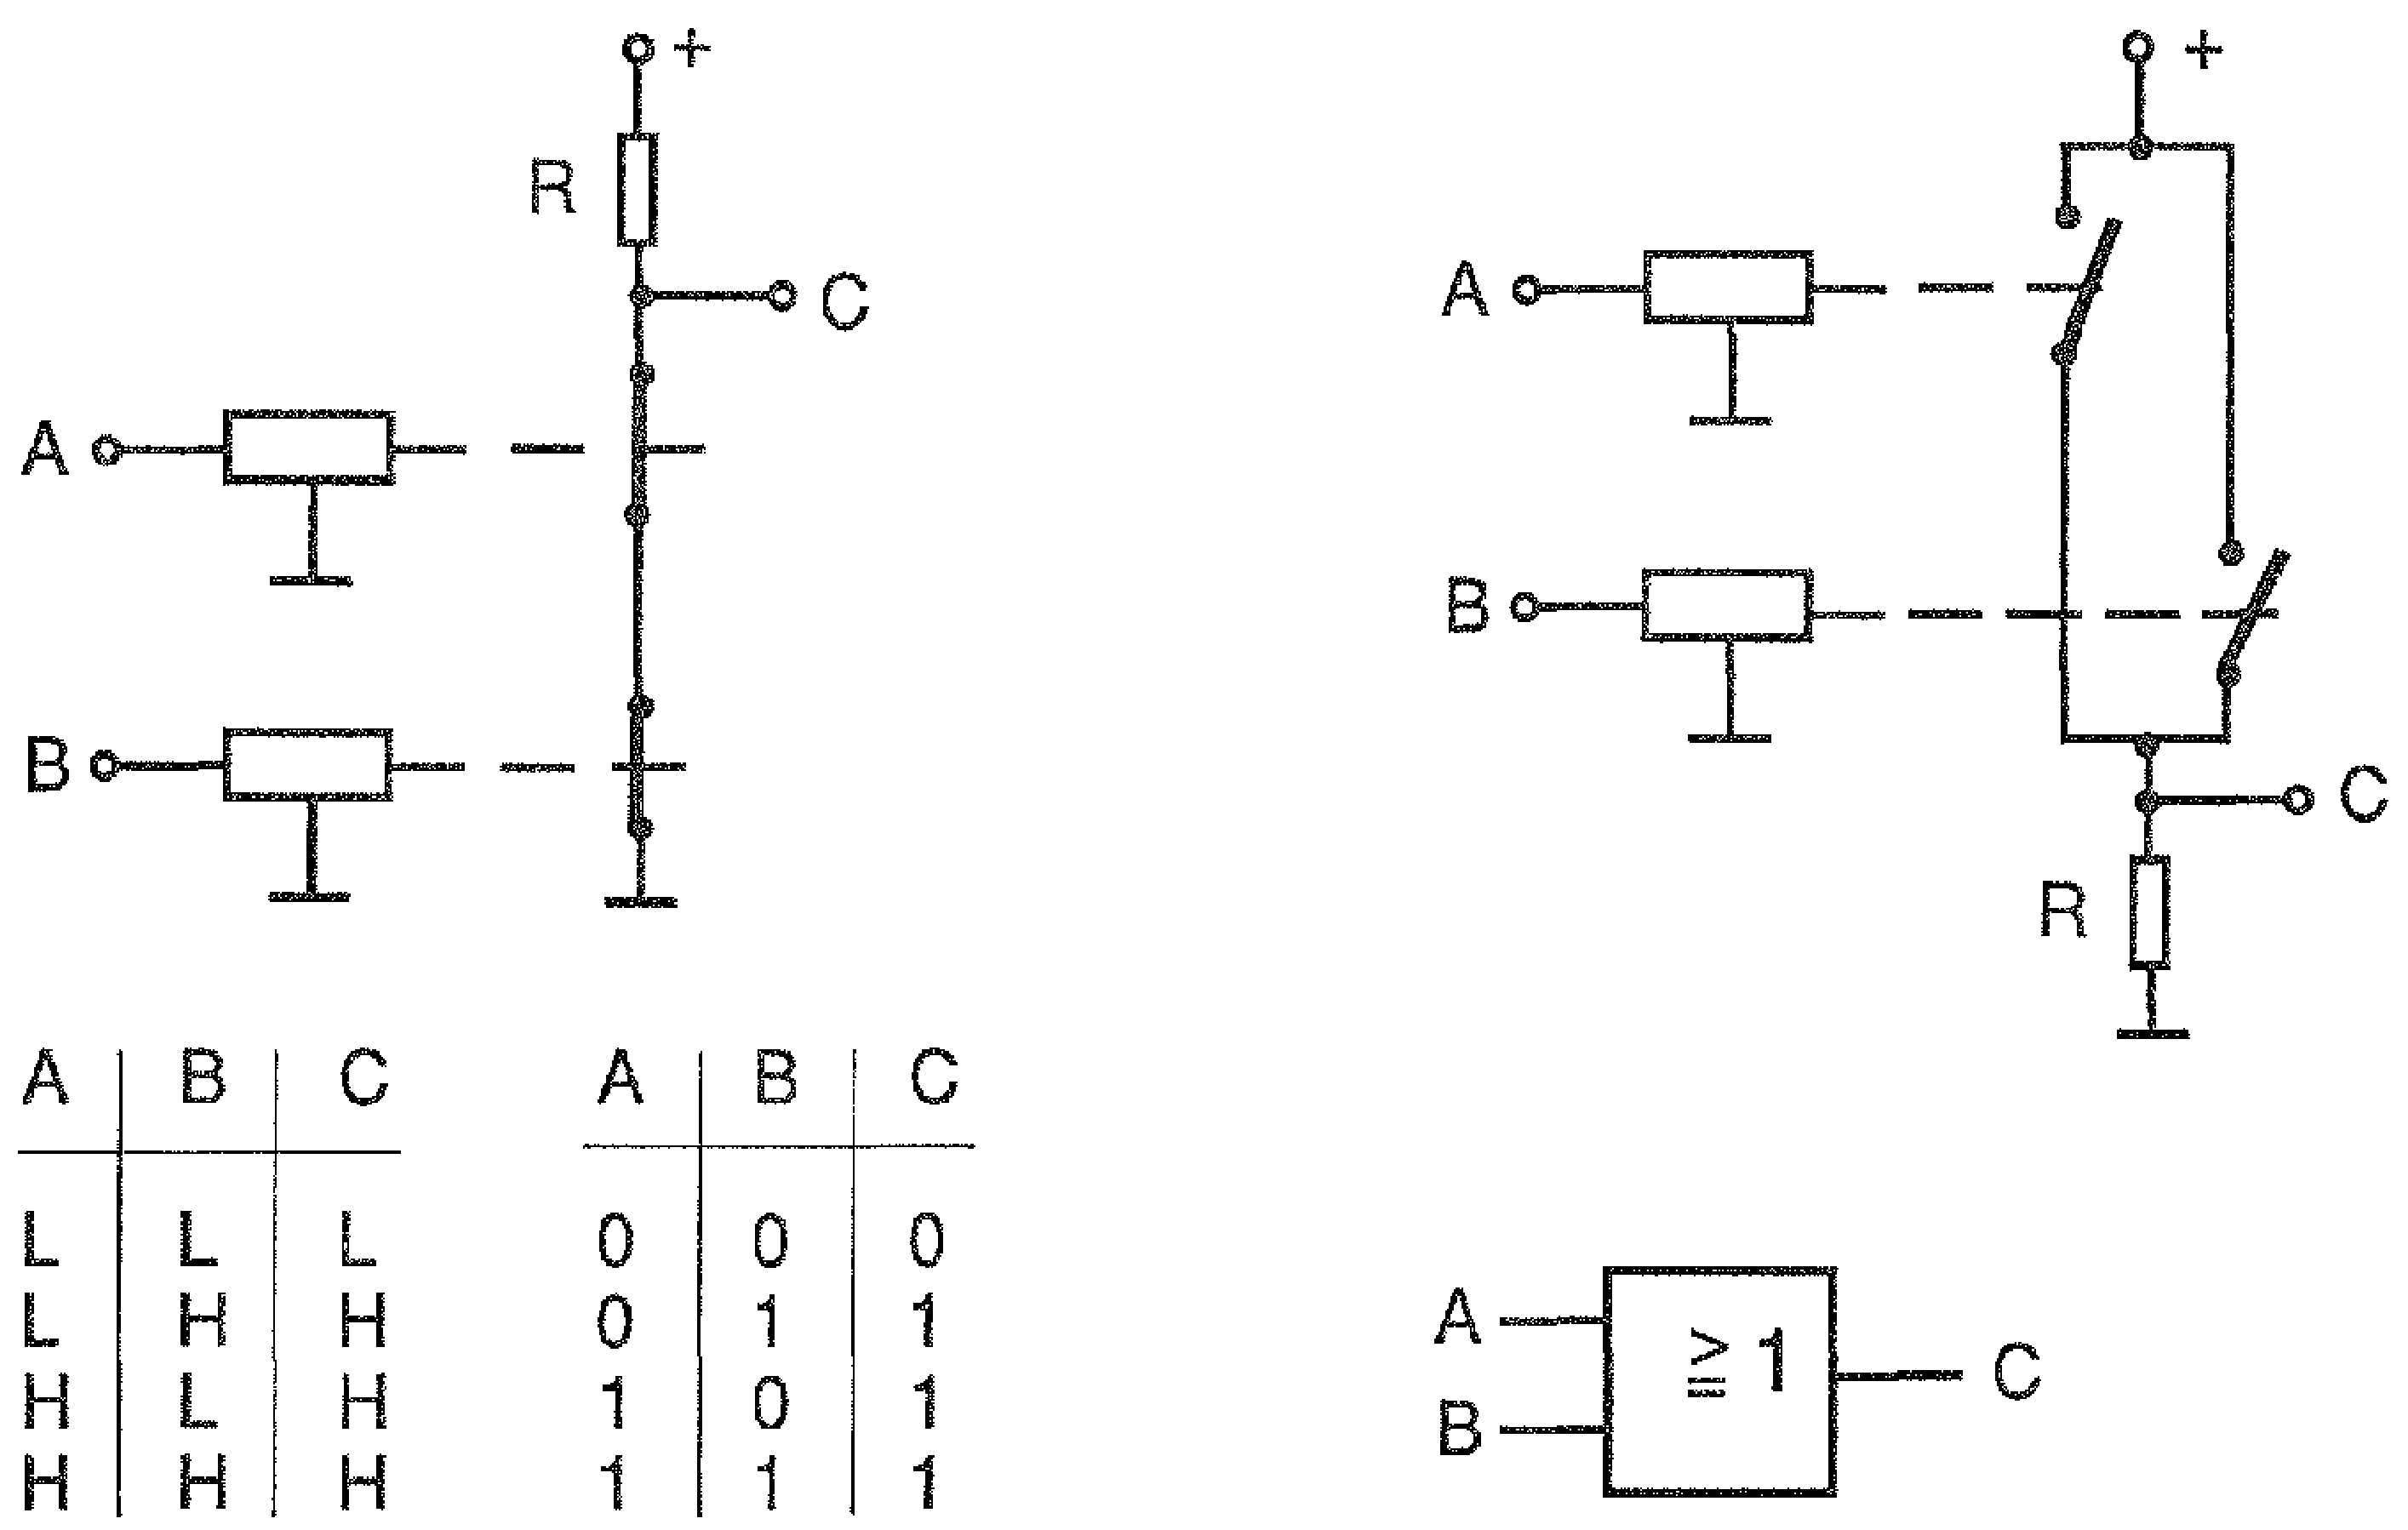
\includegraphics[width=\textwidth]{images/cropped_pdfs/bild_2_2-38.pdf}
\caption{ELLER-grind (OR-gate)}
\label{fig:BildII2-38}
\end{figure}

Sanningstabellen i bild \ref{fig:BildII2-38} säger att när en eller
flera av insignalerna är 1 så är utsignalen också 1. När alla
insignaler är 0 är utsignalen 0.

\subsubsection{OCH INTE-grind eller NAND-gate}
\index{NAND-gate}

\begin{figure}
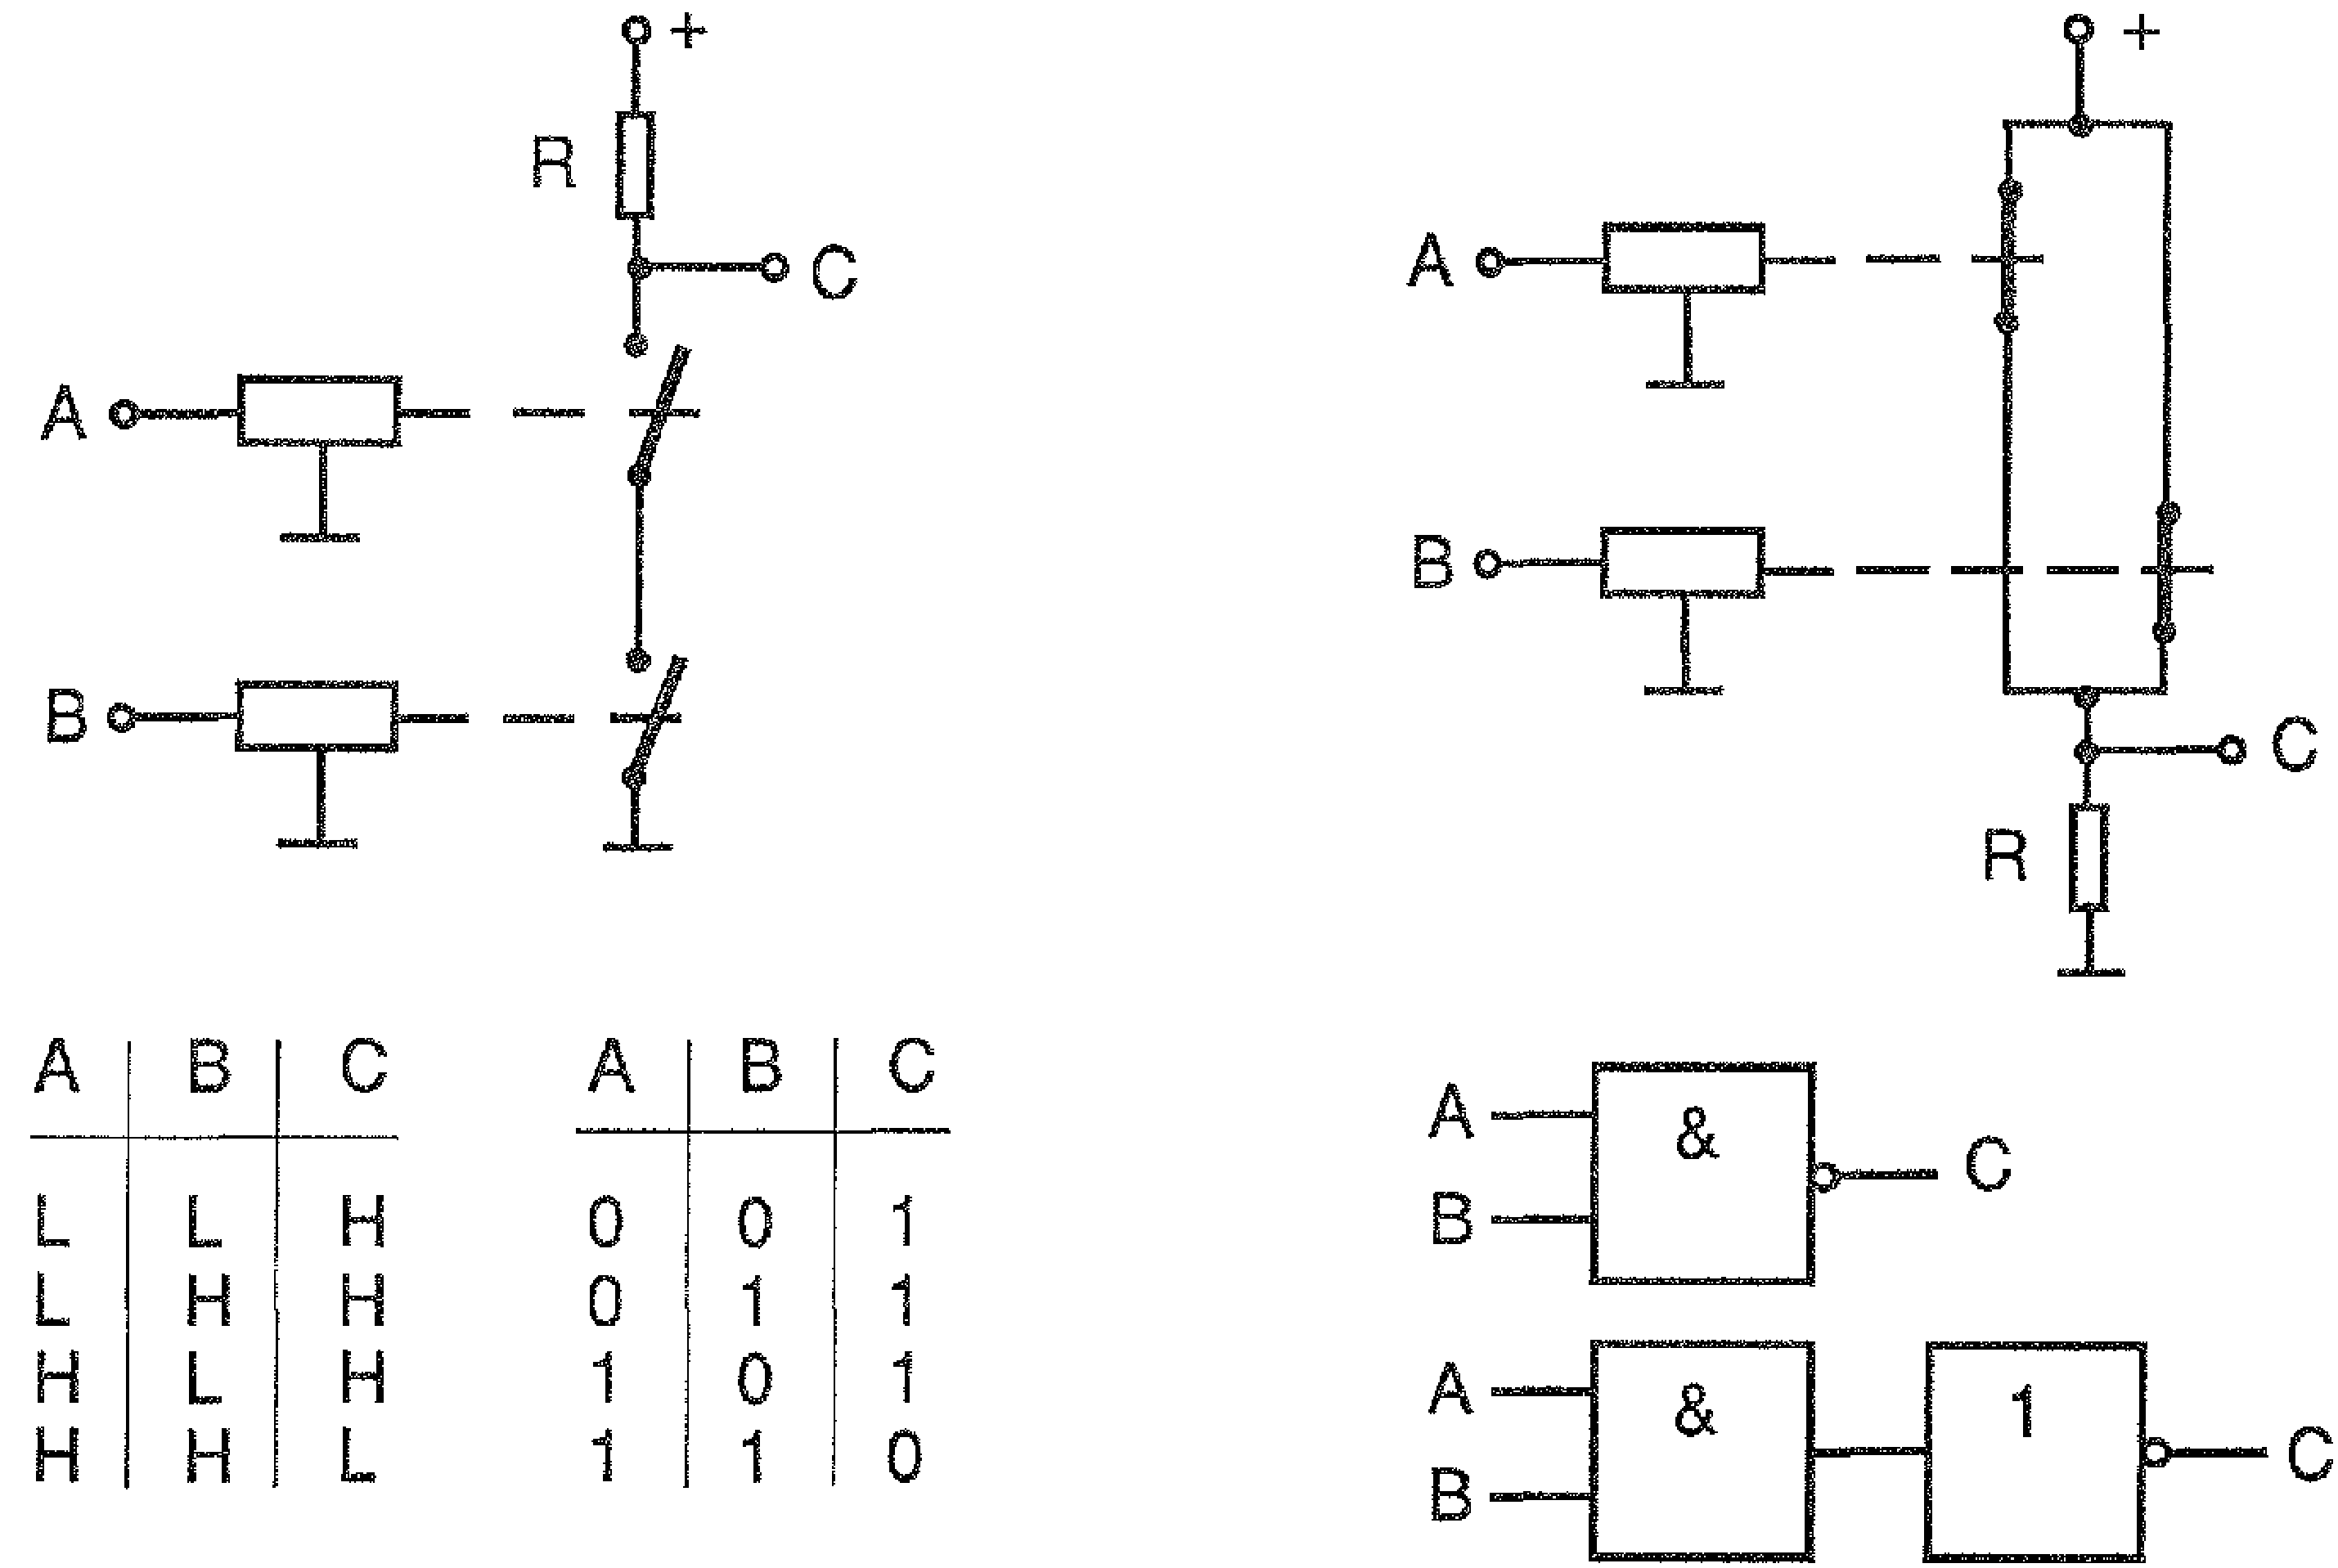
\includegraphics[width=\textwidth]{images/cropped_pdfs/bild_2_2-39.pdf}
\caption{OCH INTE-grind (NAND-gate)}
\label{fig:BildII2-39}
\end{figure}

Sanningstabellen i bild \ref{fig:BildII2-39} säger att när ingen eller
någon insignal är 1, men inte alla, så är utsignalen 1. När alla
insignaler är 1 är utsignalen 0.

\subsubsection{INTE ELLER-grind eller NOR-gate}
\index{NOR-gate}

\begin{figure}
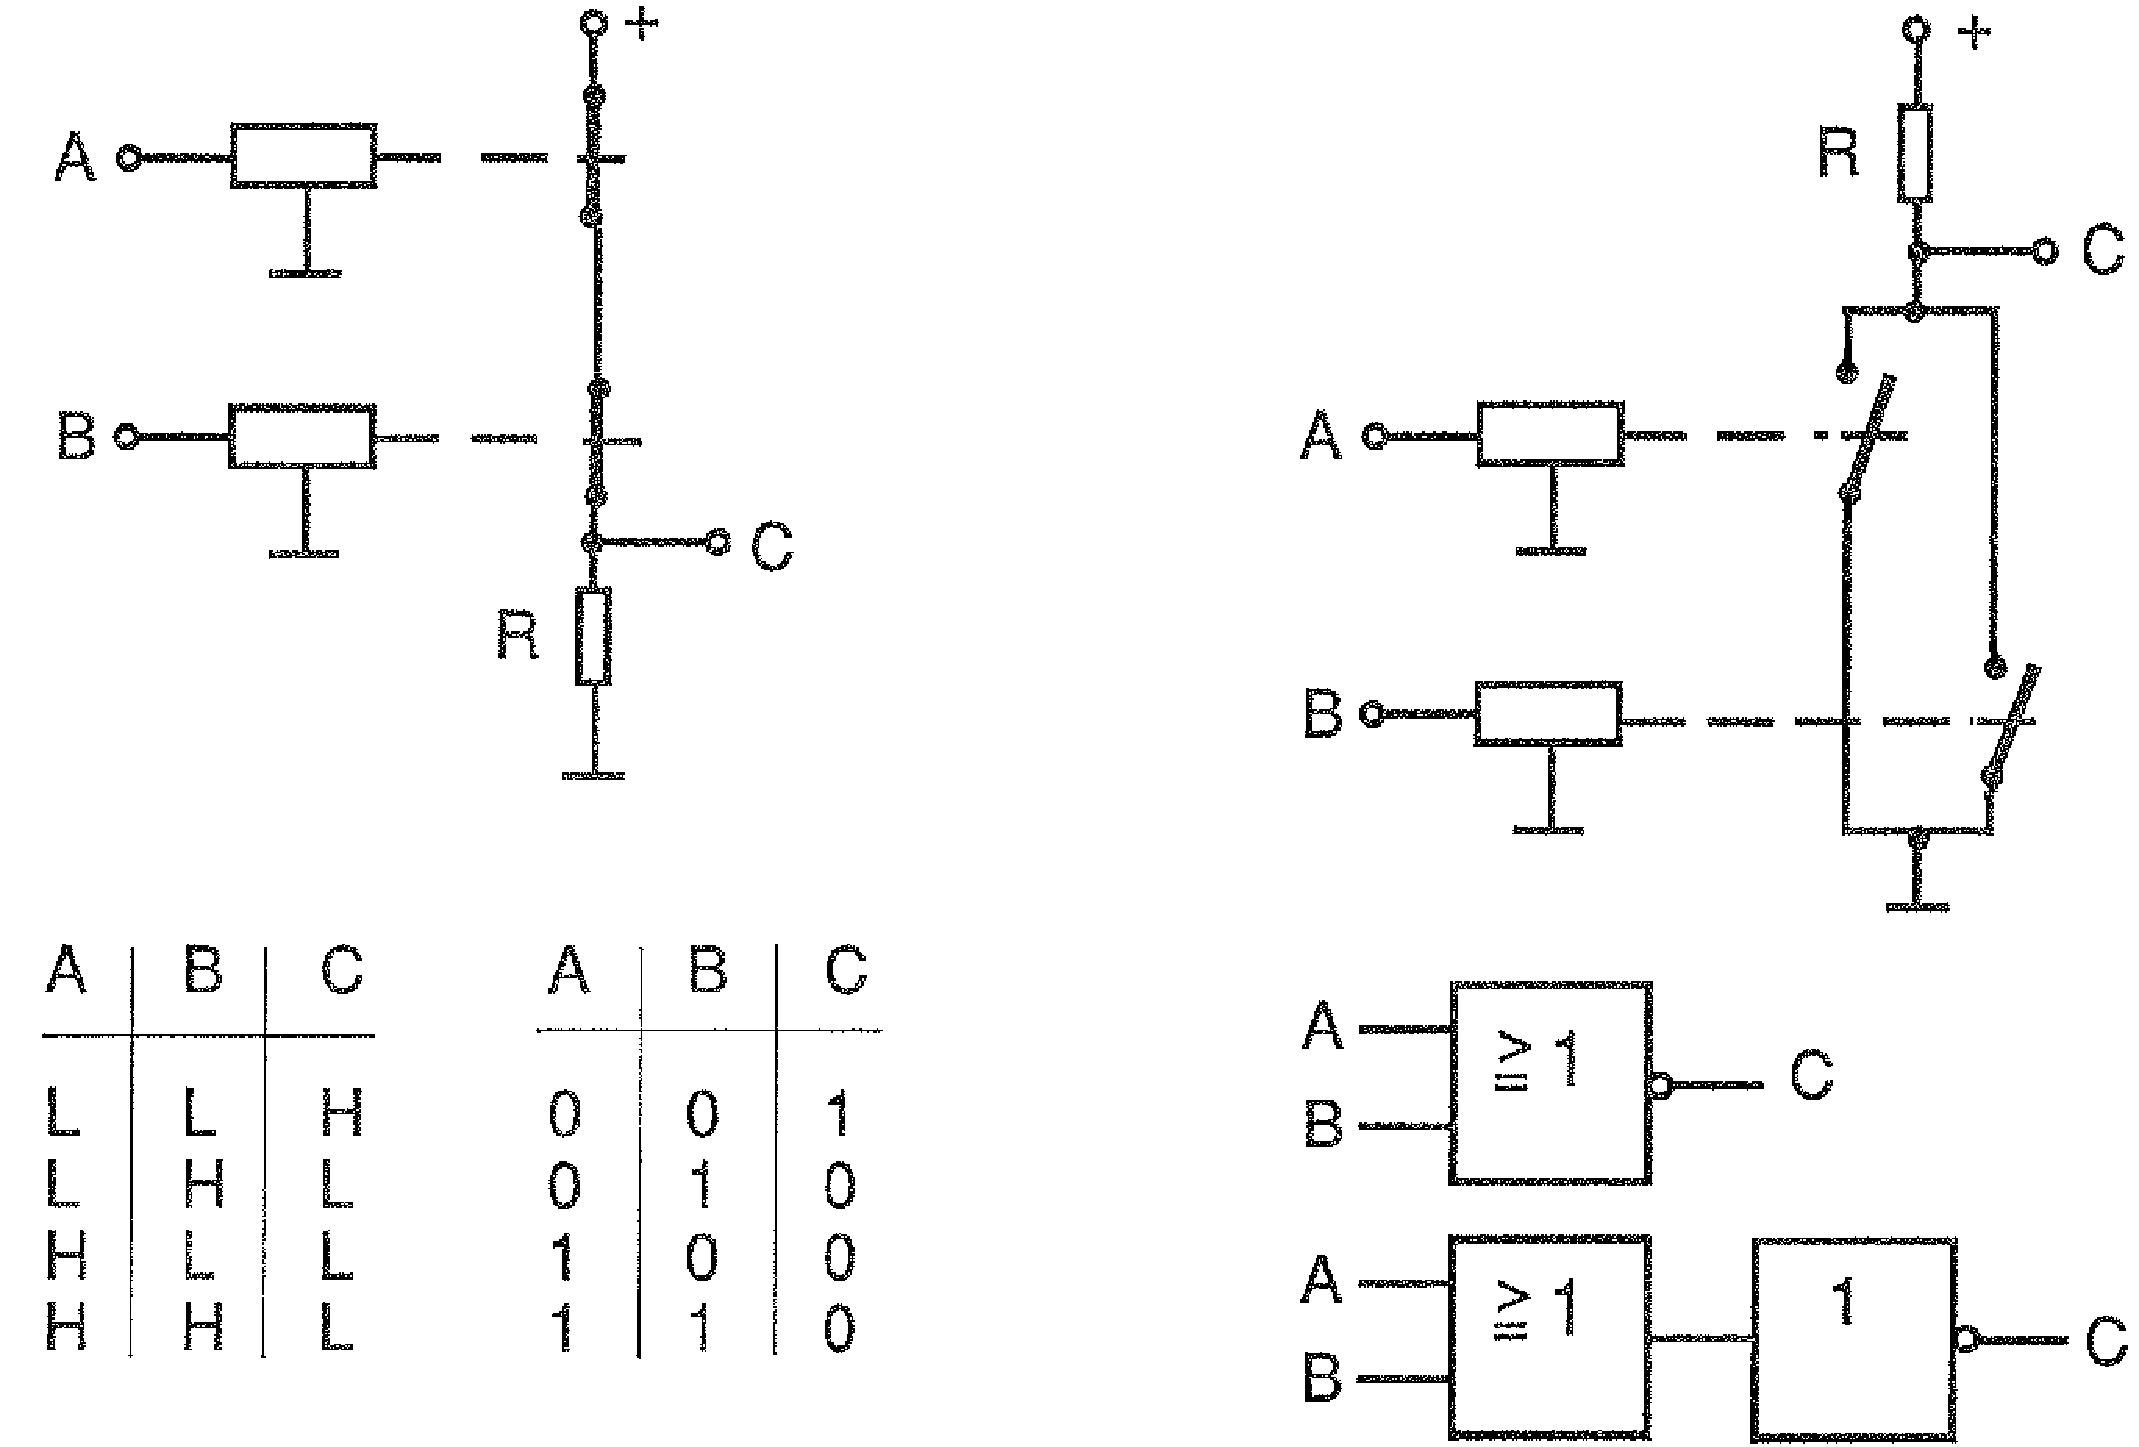
\includegraphics[width=\textwidth]{images/cropped_pdfs/bild_2_2-40.pdf}
\caption{INTE ELLER-grind (NOR-gate)}
\label{fig:BildII2-40}
\end{figure}

Sanningstabellen i bild \ref{fig:BildII2-40} säger att när någon eller alla
insignaler är 1 är utsignalen 0.
När alla insignaler är 0 är utsignalen 1.

\subsubsection{Inverterad ingång}

En ingång kan behöva ha en inverterad funktion i förhållande till de
övriga (\emph{low active}). Man kan då göra som i exemplet med en
OCH-grind i bild \ref{fig:BildII2-41}.

\begin{wrapfigure}{r}{.5\textwidth}
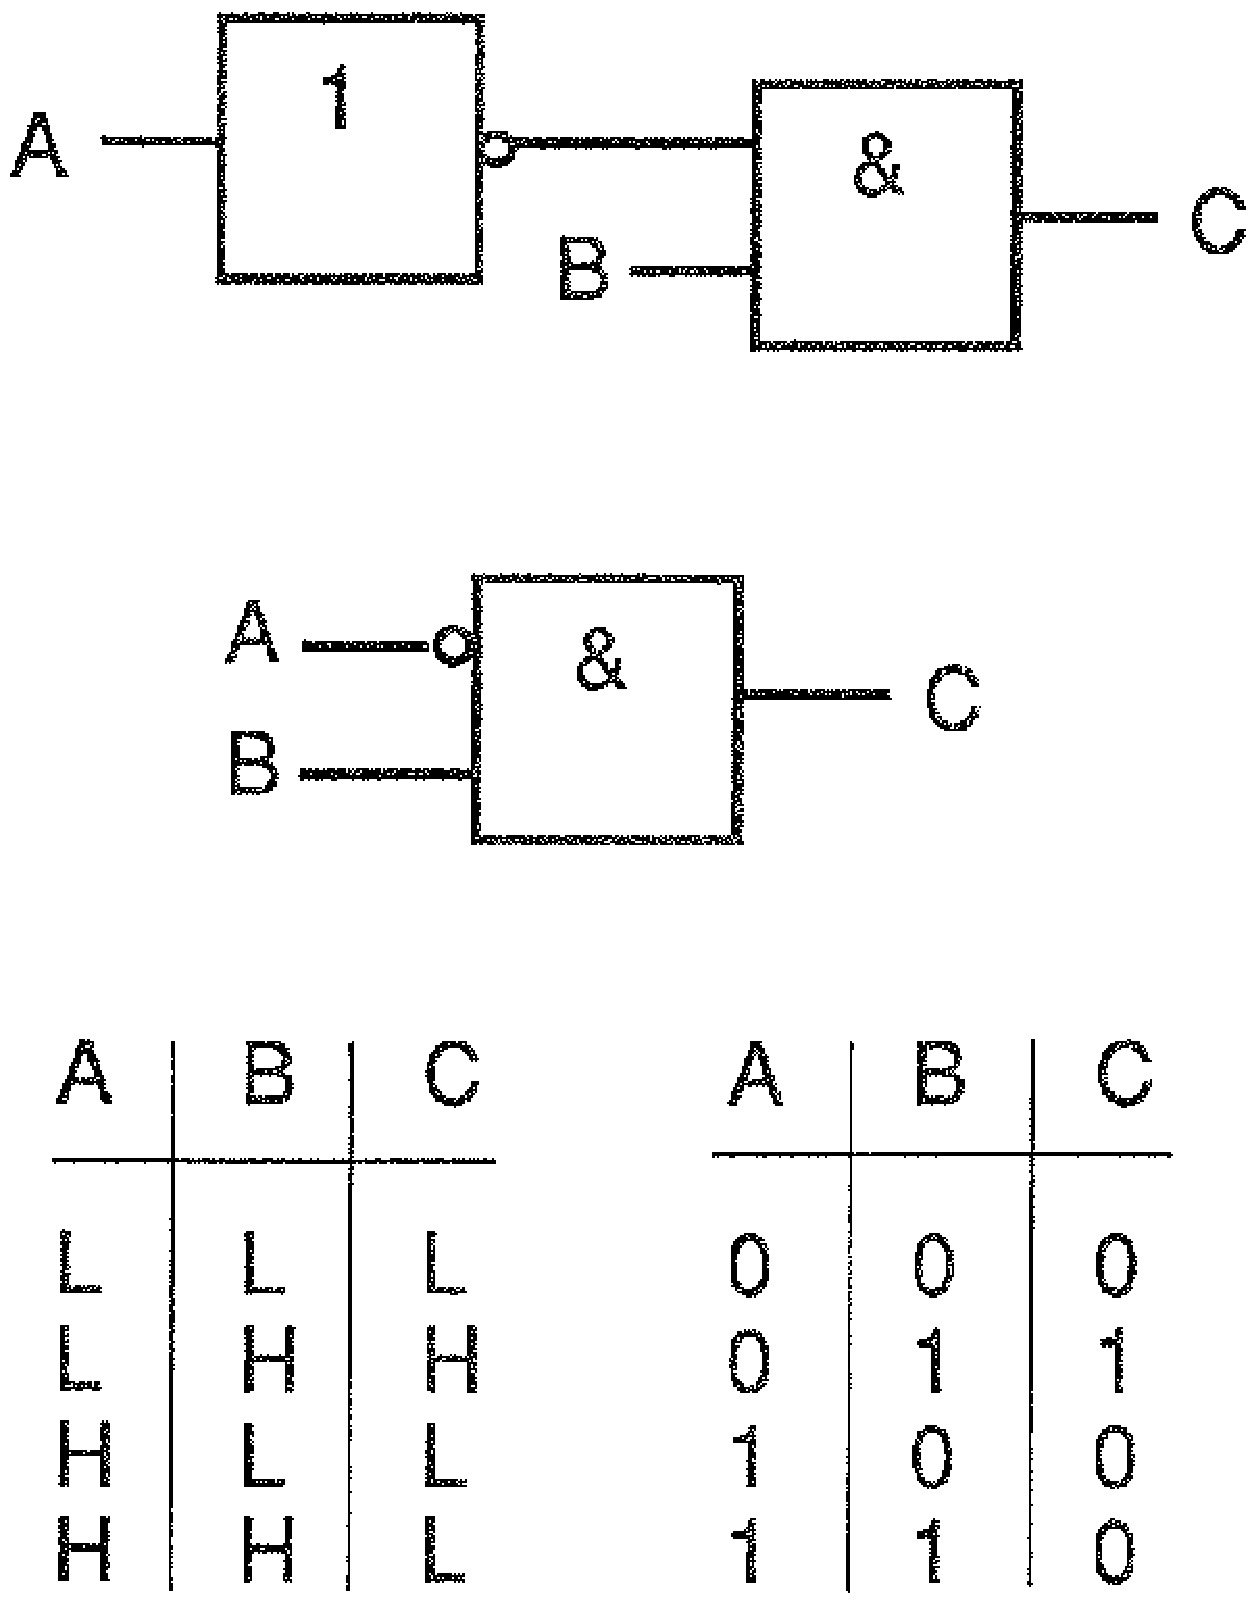
\includegraphics[width=.4\textwidth]{images/cropped_pdfs/bild_2_2-41.pdf}
\caption{Inverterad ingång}
\label{fig:BildII2-41}
\end{wrapfigure}

\subsubsection{Exklusiv ELLER-grind (XOR-gate)}
\index{XOR-gate}

Sanningstabellen i bild \ref{fig:BildII2-42} säger att när alla
insignaler antingen är 1 eller 0, så är utsignalen 0. När någon
insignal är 1, men inte alla, så är utsignalen 1.

\begin{marginfigure}%{R}{.5\textwidth}
  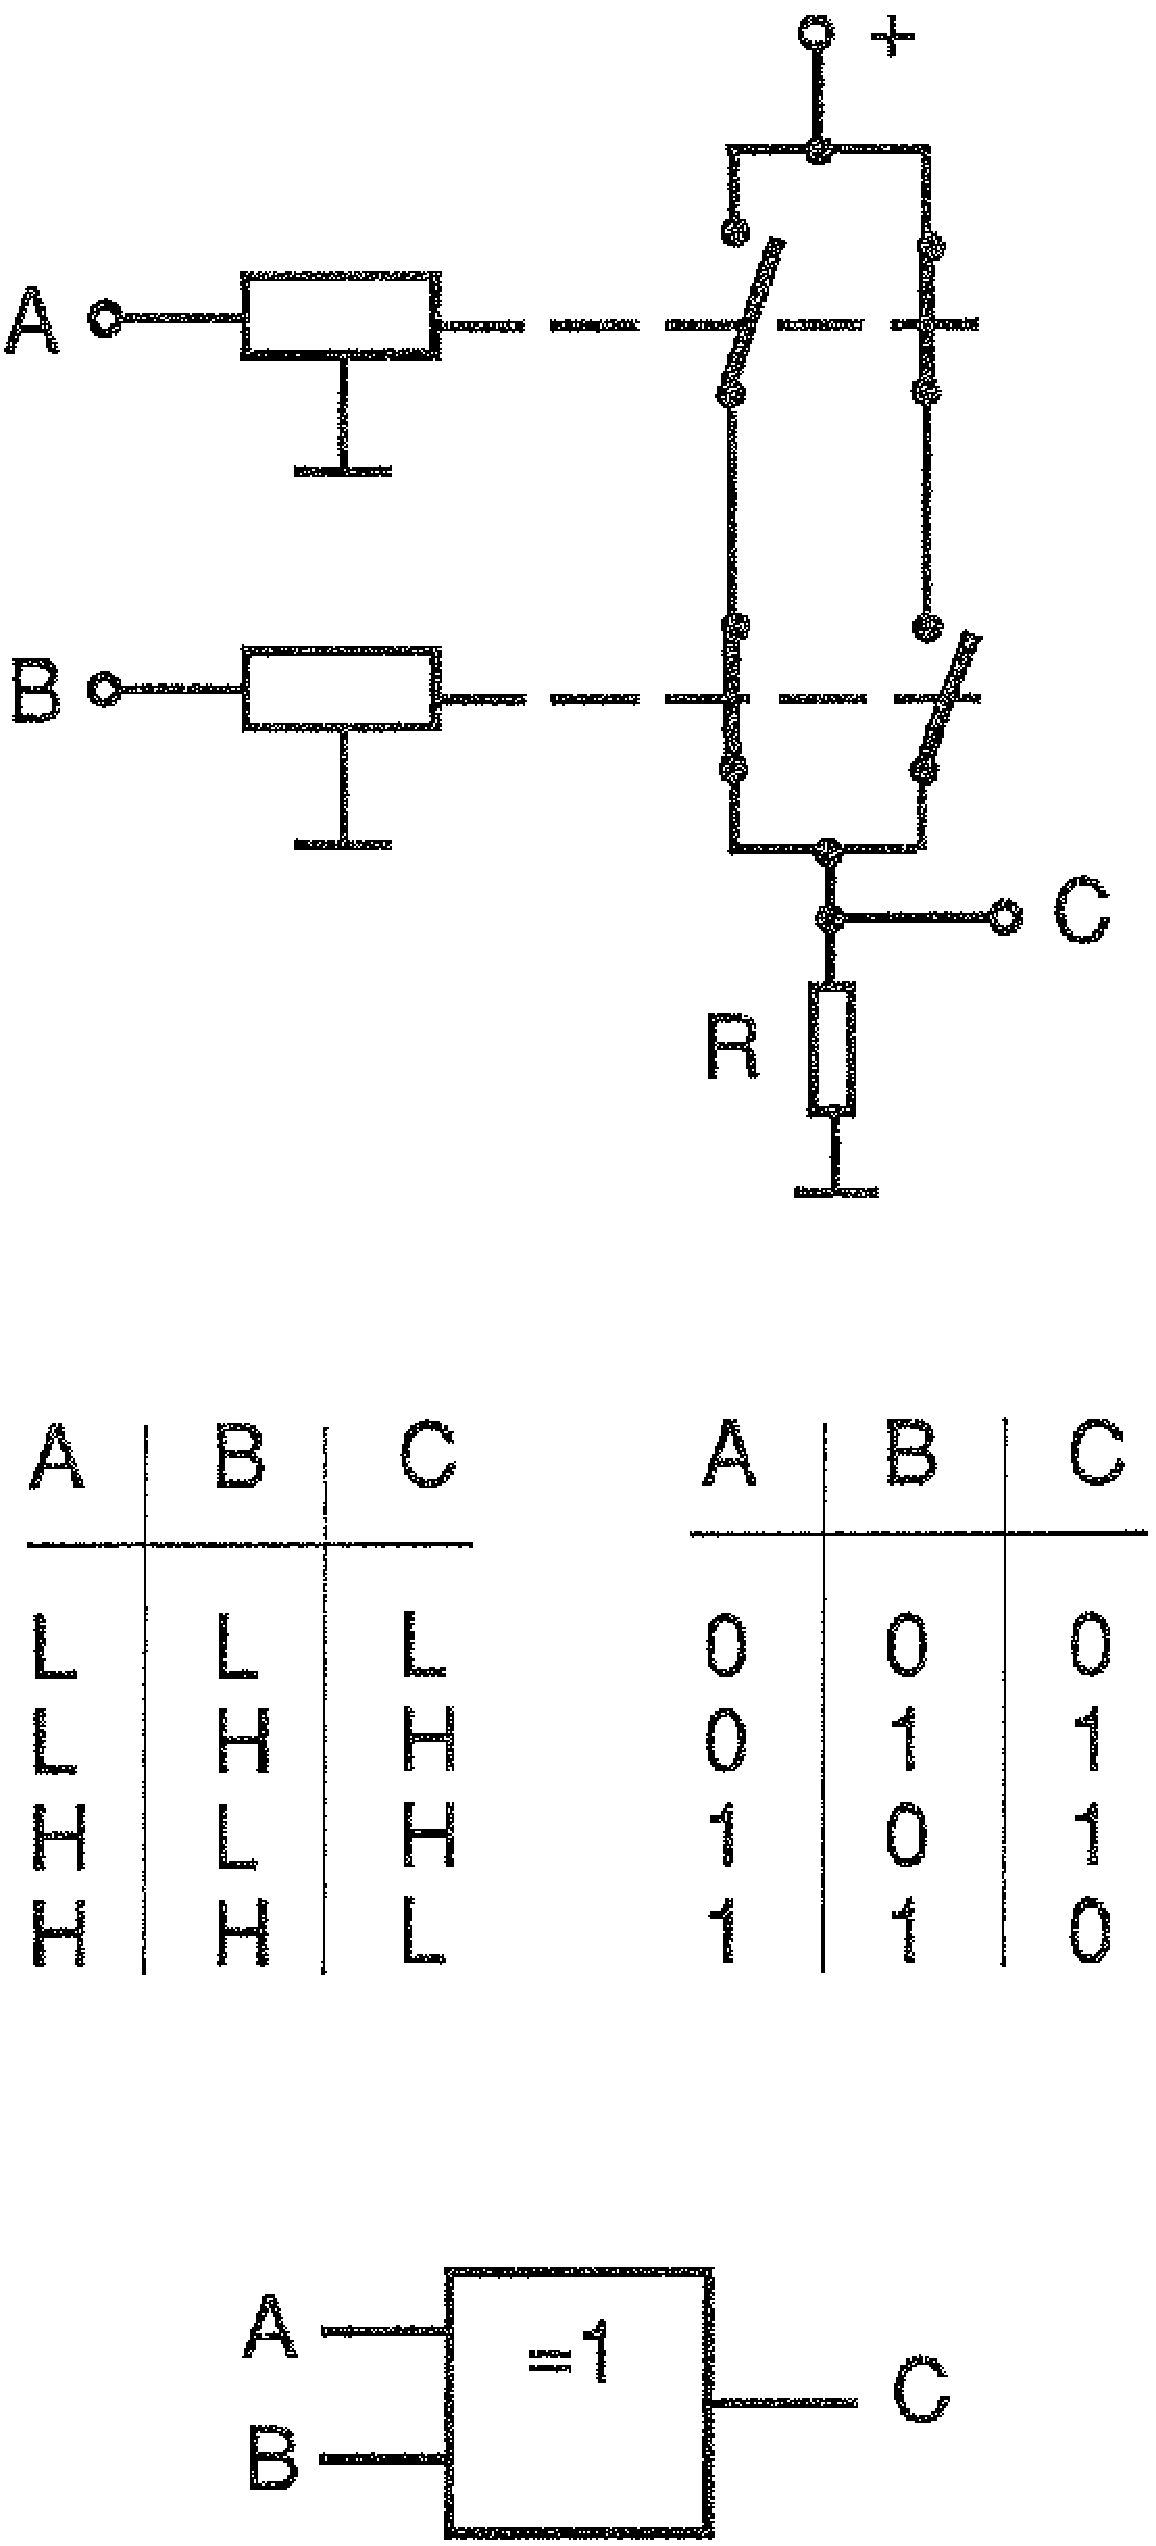
\includegraphics[width=.7\textwidth]{images/cropped_pdfs/bild_2_2-42.pdf}
  \caption{Exklusiv ELLER-grind (EXOR-gate)}
  \label{fig:BildII2-42}
\end{marginfigure}


\subsubsection{Exklusiv INTE ELLER-grind (XNOR-gate)}
\index{XNOR-gate}

Sanningstabellen i bild \ref{fig:BildII2-43} säger, att när alla insignaler
antingen är 1 eller 0, så är utsignalen 1.
När en, men inte alla insignaler är 1, så är utsignalen 0.

\subsection{Grindar med dioder och transistorer}

I stället för reläer eller diskreta halvledare i grindar använder man nu ytterst sällan något annat än integrerade digitala kretsar (se avsnitt \ref{integrerade kretsar}).

\begin{figure}%{R}{.25\textwidth}
	\centering
	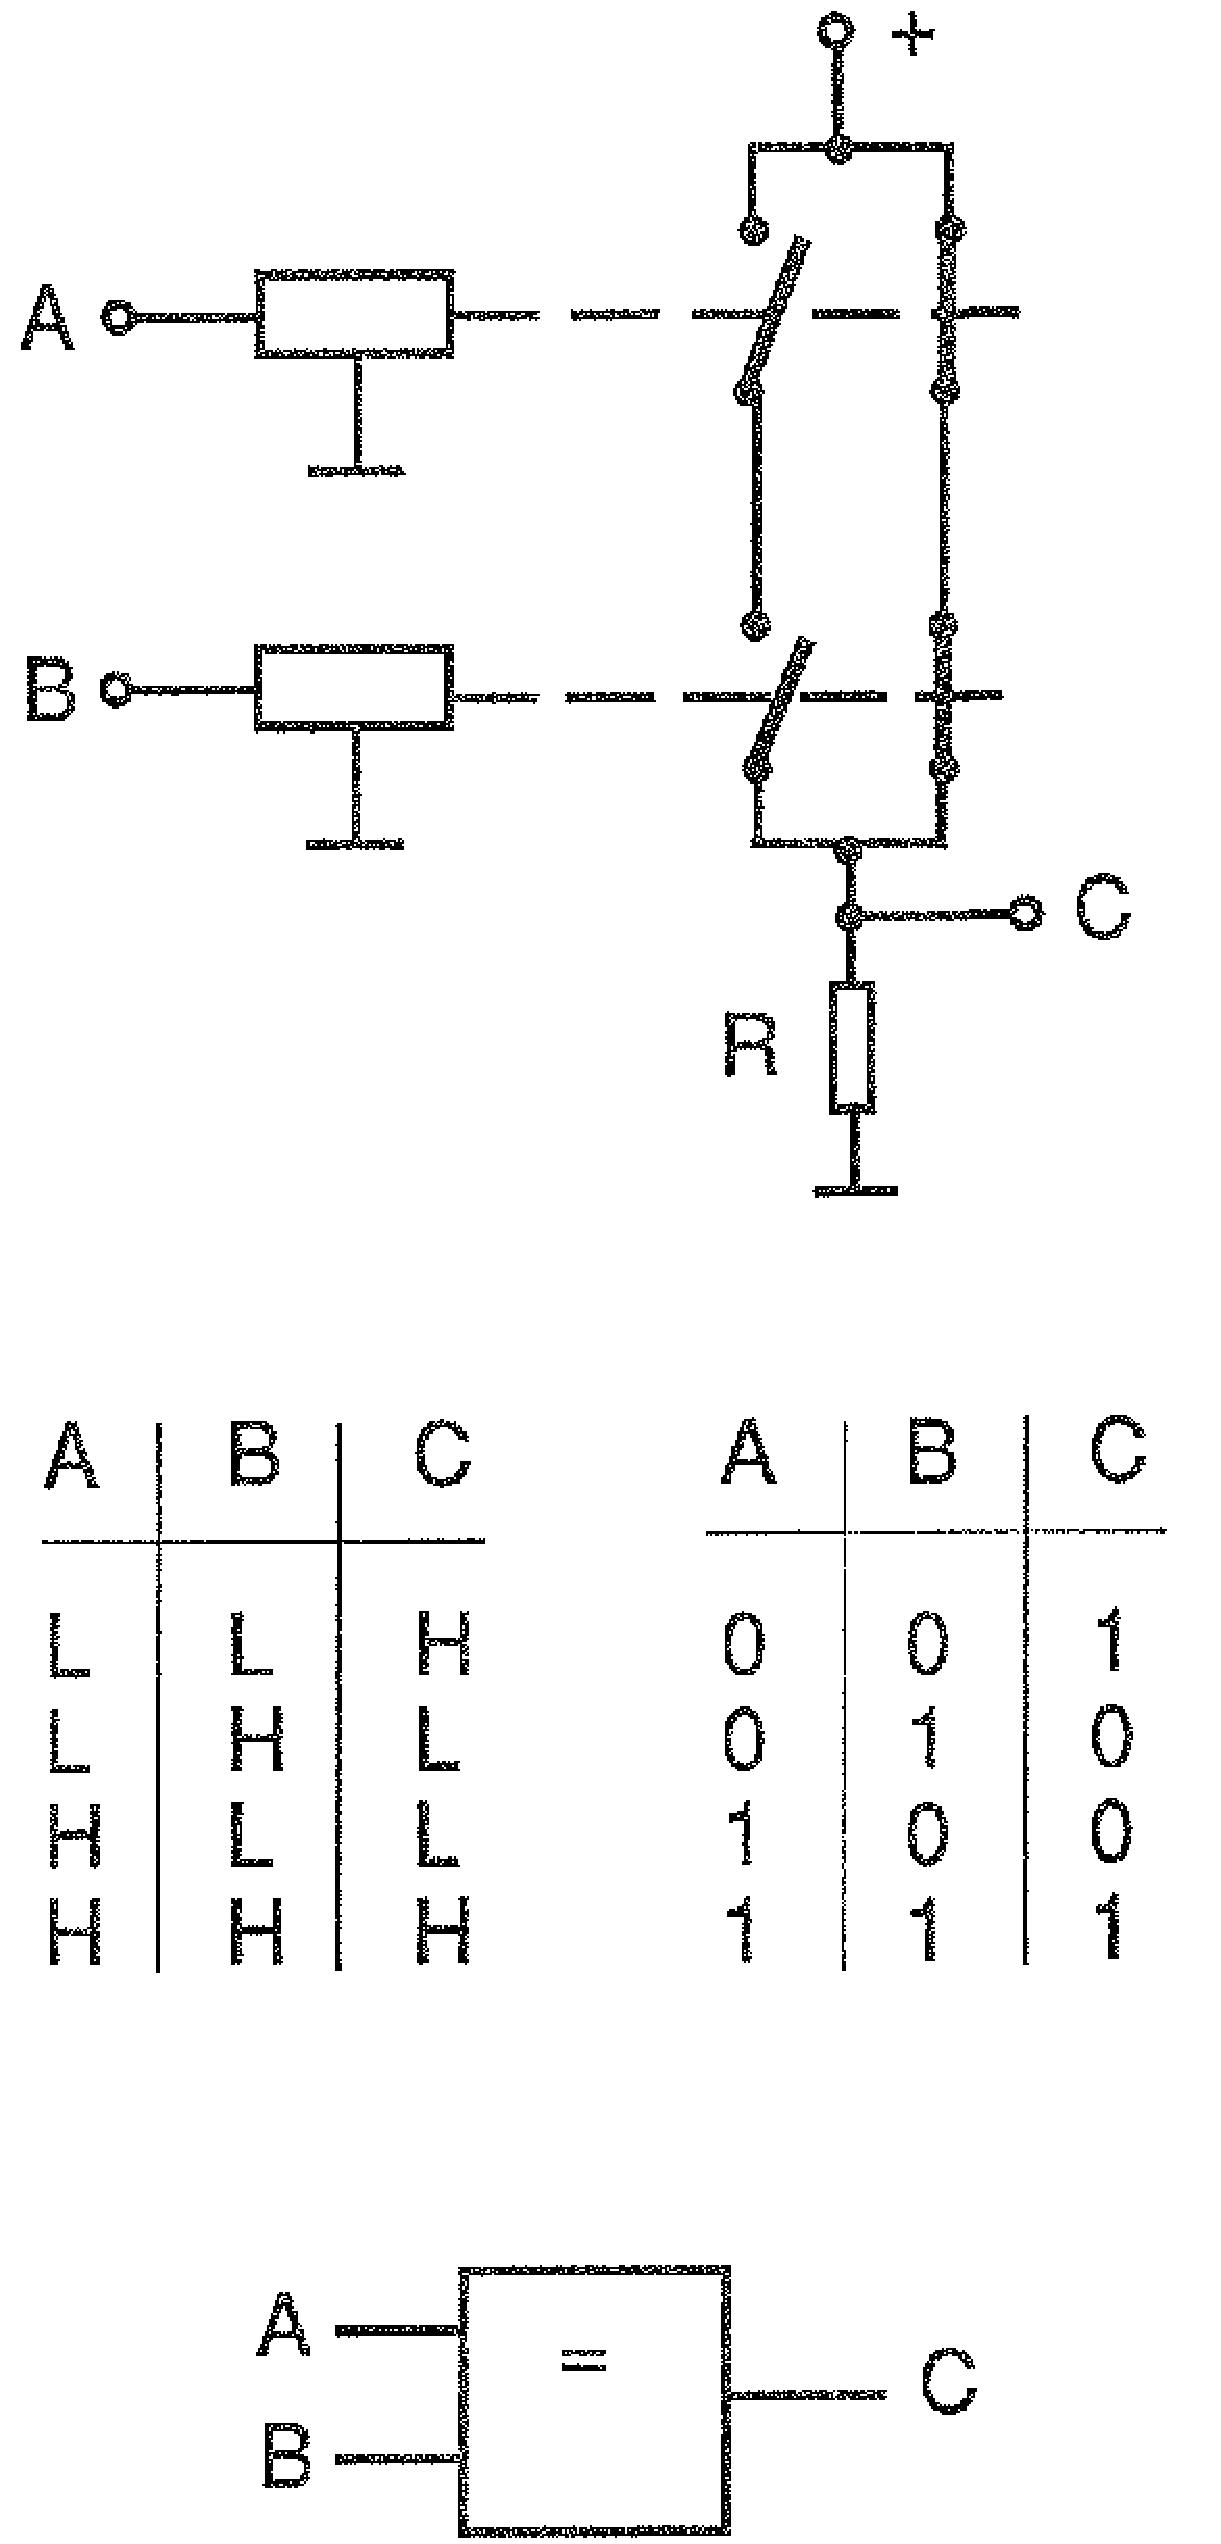
\includegraphics[width=.3\textwidth]{images/cropped_pdfs/bild_2_2-43.pdf}
	\caption{Exklusiv INTE ELLER-grind (EXNOR-gate)}
	\label{fig:BildII2-43}
\end{figure}

\begin{marginfigure}
	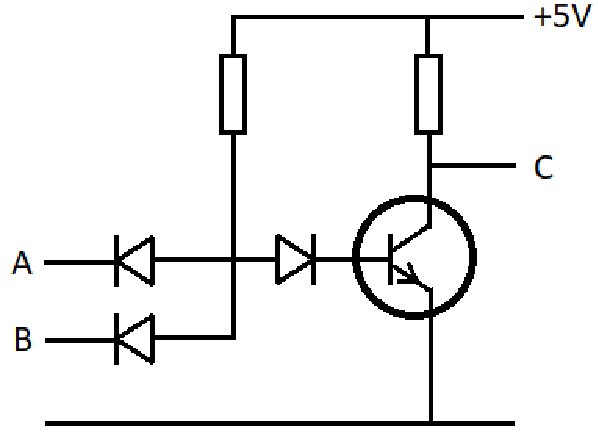
\includegraphics[]{images/cropped_pdfs/bild_2_2-44.pdf}
	\caption{DTL-logik}
	\label{fig:BildII2-44}
\end{marginfigure}

\begin{marginfigure}
	\vspace{\baselineskip}
	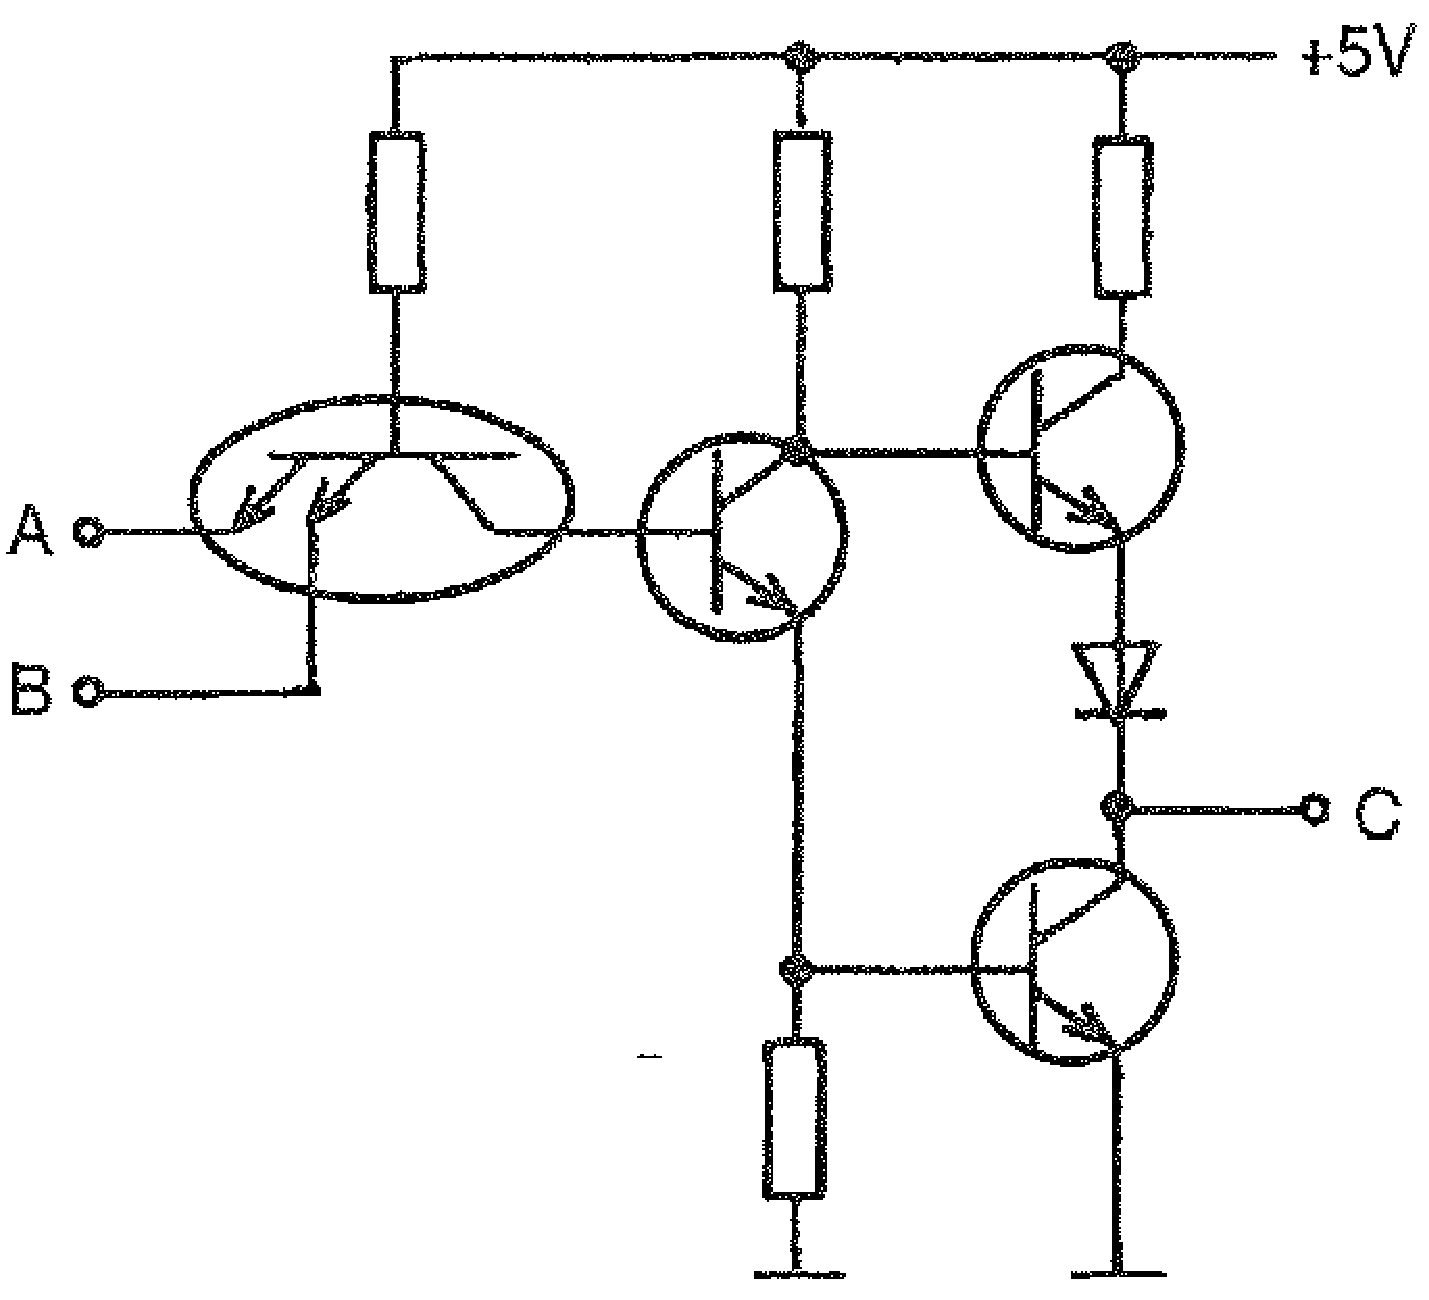
\includegraphics[]{images/cropped_pdfs/bild_2_2-45.pdf}
	\caption{TTL-logik}
	\label{fig:BildII2-45}
\end{marginfigure}

Bild \ref{fig:BildII2-44} visar en NAND-grind.
Den egentliga grinden består av tre dioder och en resistor.
Två av dioderna är ingångar och den tredje är utgång.
Grinden styr en digitalt arbetande transistor liksom den i bild
\ref{fig:BildII2-35}.
Resultatet är en så kallad DTL-logik (eng. \emph{Diode-Transistor Logic}).

Bild \ref{fig:BildII2-45} visar en NAND-grind.
Här består den egentliga grinden av en ingångstransistor med två emittrar,
vilka motsvarar dioderna vid A och B i föregående bild.

Kollektorn i denna transistor motsvarar ingångsdioden till transistorn i bild
\ref{fig:BildII2-44}.
De övriga tre transistorerna i bild \ref{fig:BildII2-45} bildar en switch (digital strömställare, jämför bild \ref{fig:BildII2-35}),
som ger snabb övergång mellan väl definierade logiska nivåer.
Resultatet är en så kallad TTL-logik (eng. \emph{Transistor-Transistor Logic}).
